
%(BEGIN_QUESTION)
% Copyright 2015, Tony R. Kuphaldt, released under the Creative Commons Attribution License (v 1.0)
% This means you may do almost anything with this work of mine, so long as you give me proper credit

Calculate all currents and voltages in this current transformer (CT) circuit:

$$\includegraphics[width=15.5cm]{i02606x01.eps}$$

\vskip 100pt

Now, calculate all currents and voltages in this current transformer circuit, with two identical CTs connected in series:

$$\includegraphics[width=15.5cm]{i02606x02.eps}$$

\vskip 100pt

Finally, sketch the direction of current through each CT assuming the direction shown by the 180 amp arrow at one particular instant in time.

\vfil 

\underbar{file i02606}
\eject
%(END_QUESTION)





%(BEGIN_ANSWER)

This is a graded question -- no answers or hints given!

%(END_ANSWER)





%(BEGIN_NOTES)

In the original circuit, the line current of 180 amps generates a secondary CT current of:

$$\left( 180 \hbox{ A} \over 1 \right) \left(5 \over 300 \right) = 3 \hbox{ A}$$

This {\bf 3 amp} secondary current passes equally through both the 0.25 $\Omega$ resistor and the 2.3 $\Omega$ burden of the protective relay, because those components are wired in series with the CT.  Ohm's Law ($V = IR$) gives us a {\bf 0.75 volt} drop across the 0.25 $\Omega$ resistor and a {\bf 6.9 volt} drop across the relay's burden, for a total voltage of {\bf 7.65 volts} across the CT secondary terminals.

\vskip 40pt

In the dual-CT circuit, the same current gets pushed through the resistances (for the same voltage drops across each), but each CT only has to generate half as much voltage as before since they're working together in series.  Thus, each CT outputs {\bf 3.825 volts} in the dual-series configuration.

\vskip 40pt

When current energizes a transformer's primary winding, it powers that winding as though it were a {\it load}.  The transformer's secondary winding, on the other hand, functions as a {\it source} to deliver power to whatever load(s) connect to it.  Since polarity marks (dots, or squares, or ``X'' marks) on transformer windings always refer to similar {\it voltages} between primary and secondary, we must view current as going in {\it opposite} directions from primary to secondary, in keeping with the view of the primary winding as a load and the secondary winding as a source.  This means the 3 amp secondary current will {\bf enter into the ``polarity'' terminal of each CT secondary winding} just as the 180 amp primary current enters into the ``nonpolarity'' terminal of each CT's primary:

$$\includegraphics[width=15.5cm]{i02606x03.eps}$$

%INDEX% Electronics review: current transformer (CT)

%(END_NOTES)


